%!TEX root = thesis.tex
\chapter{Method}
\section{Experimental setup}
\subsection{ALICE Experiment}
A description of the ALICE detector\ref{fig:alice_detector} and its performance are reported in Refs.~\cite{Alice_performance,Aamodt:2008zz}. 
The data used for these analyses were recorded with a minimum-bias trigger, based on coincident signals in the two scintillator arrays (V0) located on both sides of the interaction vertex.
Offline selections, based on the V0 and Silicon Pixel Detector signals~\cite{Reidt:2151986}, were applied to remove background from beam--gas collisions.
Pile-up events (less than 1\%) containing multiple primary vertices were rejected.
Only events with a reconstructed primary vertex position within $\pm$10~cm in the longitudinal direction from the nominal centre of the detector were used.
With these requirements, $1.9 \times 10^9$ pp events were selected, corresponding to an integrated luminosity of $\mathcal{L}_{\rm int}=$~32.95 $\pm$ 1.65~${\rm nb^{-1}}$.

\begin{figure}[!htb]
    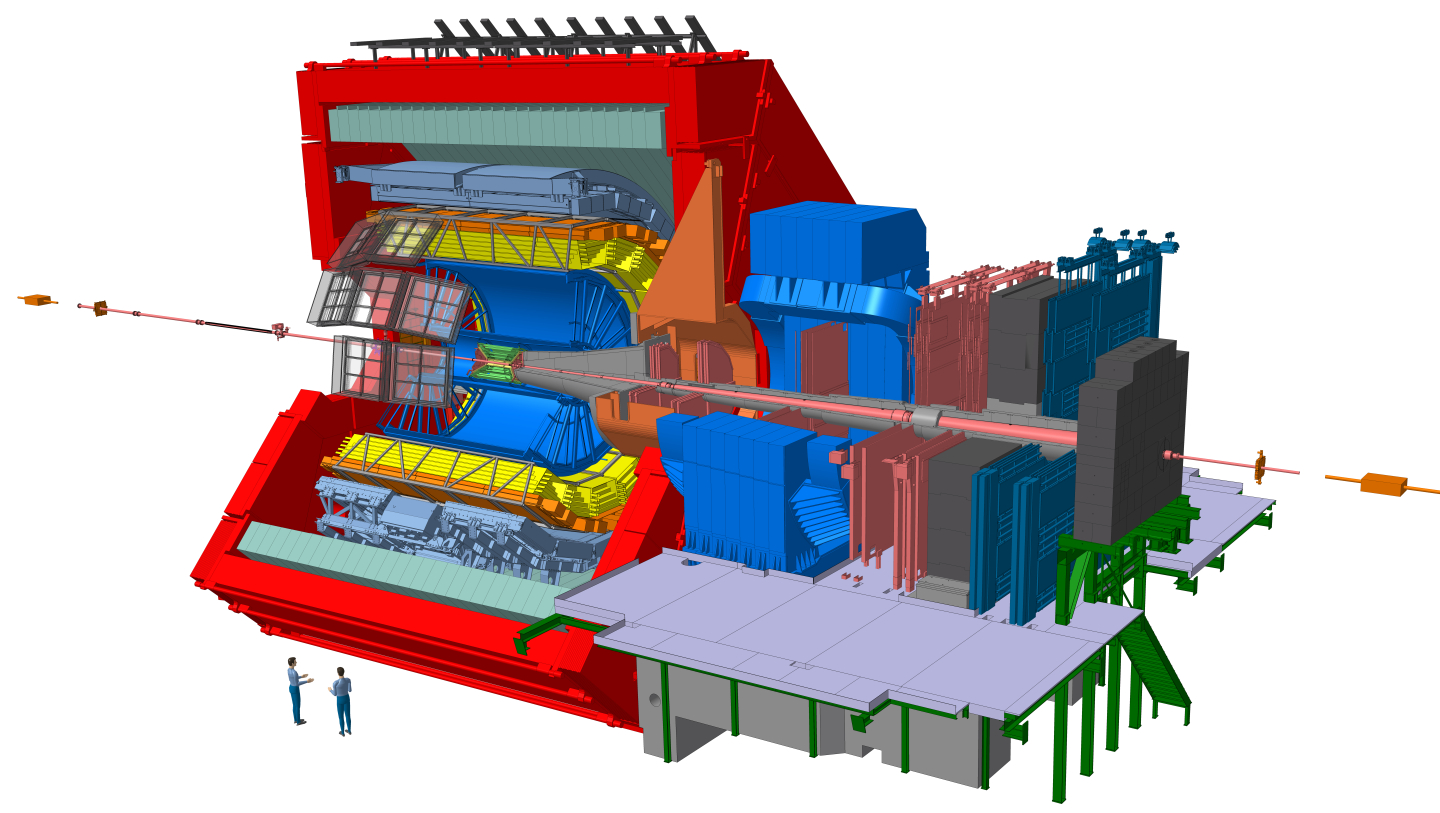
\includegraphics[width=0.85\textwidth]{fig/alice_detector_no_ITS.jpg}
    \caption{\it ALICE detector}
    \label{fig:alice_detector}
\end{figure}
    